% !TEX root = ../main.tex

\appendix
\chapter{Entrevistas}
	\begin{itemize}
		\item \textbf{Entrevista realizada dia 16 de outubro de 2014}

			\cliente~ George Marsicano

			Foi planejado pela equipe de desenvolvimento uma entrevista superficial com seis perguntas, porêm, após a primeira pergunta respondida não foi mais necessário as outras perguntas, salvo a pergunta de número dois.

			São elas:			

			\textbf{1. Por que criar uma nova ferramenta de requisitos? As existentes nao te agradram?}
		
			\textbf{R:} Não me agradam?

			A necessidade de criação ou não de uma ferramenta não vem da necessidade de ferramente em si.
			
			Vocês em primeiro passo estão modelando um processo de requisitos. Depois será realizado uma avaliação para saber se existe ou não alguma ferramenta que implemente este processo definido, e, por ultimo, caso não exista nenhuma ferramente, poderá ser desenvolvido um plug-in para alguma existente que seja possível tal adaptação, ou o desenvolvimento de uma nova ferramente por completo.
			
			Tudo dependerá a modelagem inicial para decidir o andamento e escopo do projeto.
		
			\textbf{2. Se fosse possível resumir a sua necessidade em uma palavra, qual seria?}

			\textbf{R:} Abrangência.
	\end{itemize}

\chapter{Priorização dos casos de uso}

Para a realização da priorização dos Casos de Uso que devem ser implementados utilizou-se uma entrevista com o cliente. A entrevista foi organizada da forma na qual as perguntas seriam apenas os nomes dos Casos de Uso e as respostas poderiam ser \textbf{Alta Prioridade}, \textbf{Média Prioridade} e \textbf{Baixa Prioridade}.

A entrevista e suas respostas estão dispostas na seguinte tabela:

\begin{table}[H]
\centering
\begin{tabular}{|p{7cm}|p{3cm}|}
%----------------------------------------------
\hline
\textbf{Manter Problema} &
\textcolor{red}{Prioridade Baixa}
\\ \hline
%----------------------------------------------
\textbf{Manter Necessidades} &
\textcolor{red}{Prioridade Baixa}
\\ \hline
%----------------------------------------------
\textbf{Manter Características} &
\textcolor{red}{Prioridade Baixa}
\\ \hline
%----------------------------------------------
\textbf{Manter Casos de Uso} &
\textcolor{red}{Prioridade Baixa}
\\ \hline
%----------------------------------------------
\textbf{Manter Temas de Investimento} &
\textcolor{red}{Prioridade Baixa}
\\ \hline
%----------------------------------------------
\textbf{Manter Épicos} &
\textcolor{red}{Prioridade Baixa}
\\ \hline
%----------------------------------------------
\textbf{Manter Features} &
\textcolor{red}{Prioridade Baixa}
\\ \hline
%----------------------------------------------
\textbf{Manter Histórias de Usuário} &
\textcolor{red}{Prioridade Baixa}
\\ \hline
%----------------------------------------------
\textbf{Manter Atributos} &
\textcolor{red}{Prioridade Baixa}
\\ \hline
%----------------------------------------------
\textbf{Manter RoadMaps} &
\textcolor{blue}{Prioridade Média}
\\ \hline
%----------------------------------------------
\textbf{Manter Rastreabilidade Horizontal entre os requisitos} &
\textcolor{blue}{Prioridade Média}
\\ \hline
%----------------------------------------------
\textbf{Manter Rastreabilidade Vertical entre os requisitos} &
\textcolor{blue}{Prioridade Média}
\\ \hline
%----------------------------------------------
\textbf{Definir Metodologia} &
\textcolor{green}{Prioridade Alta}
\\ \hline
%----------------------------------------------
\textbf{Definir “hibridez” do projeto} &
\textcolor{green}{Prioridade Alta}
\\ \hline
%----------------------------------------------
\textbf{Manter processos híbridos} &
\textcolor{green}{Prioridade Alta}
\\ \hline
%----------------------------------------------
\textbf{Gerar Diagrama de Ishikawa} &
\textcolor{red}{Prioridade Baixa}
\\ \hline
%----------------------------------------------
\textbf{Gerar Diagramas de Casos de Uso} &
\textcolor{blue}{Prioridade Média}
\\ \hline
%----------------------------------------------
\textbf{Gerar plano de iteração} &
\textcolor{red}{Prioridade Baixa}
\\ \hline
%----------------------------------------------
\textbf{Controlar histórico de versão} &
\textcolor{red}{Prioridade Baixa}
\\ \hline
%----------------------------------------------
\end{tabular}
\caption{Entrevista Priorização de Casos de Uso}
\label{tab:entrevista_priorizacao_uc}
\end{table}

\chapter{Ferramenta}

A seguir nas figuras de \ref{img:primeira_pag_fer} a \ref{img:primeira_pag_dps} seguem as imagens de como a ferramenta está implementada, sua interface e seu funcionamento

Inicialmente a página mostrará apenas uma apresentação da ferramenta que ainda não está implementada, e no canto superior esquero deverá apresentar ``\textit{Hello} <nome do usuário>'', porém ainda não foi implementado o login, impedindo ter uma conta de um usuário para ser colocado no nome, resultando apenas no ``\textit{Hello}''.

No menu do \textit{header} pode-se ver também um menu escrito ``\textit{New project}'' que irá direcionar o usuário para o questionário de criação de um novo projeto, e o botão ``\textit{Your projects}'' que é um menu \textit{drop down} onde serão listados todos os projetos do usuário.

Mais a direita na tela está visível o botão ``\textit{Log out}'', onde o usuário irá sair da aplicação, porém ainda não está implementado devido ao mesmo problema relatado acima na questão do campo ``\textit{Hello}'', assim como é possível visualizar na Figura \ref{img:primeira_pag_fer}.

\begin{figure}[H]
	\centering
	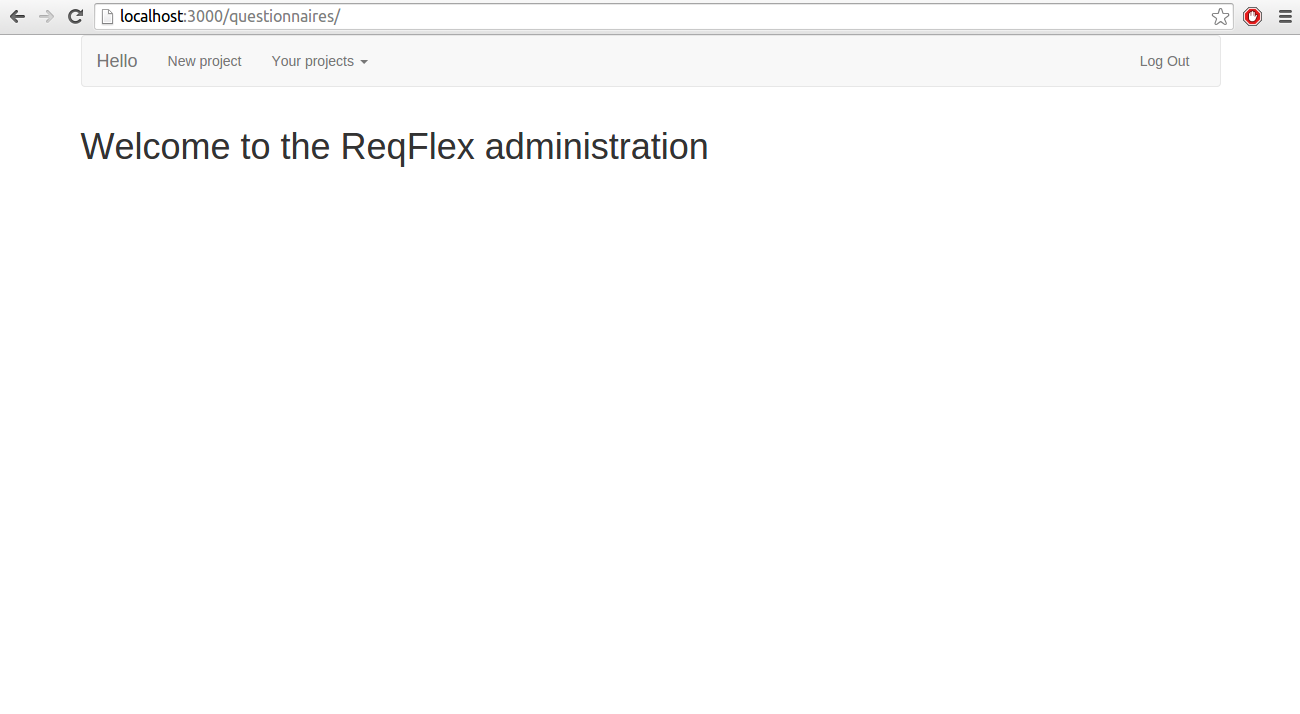
\includegraphics[scale=0.3]{imgFerramenta/primeiraPagina}
	\caption{Primeira página da ferramenta}
	\label{img:primeira_pag_fer}
\end{figure}

Após o usuário clicar sobre o botão ``\textit{New project}'' ele será redirecionado para a página que contém o formulário com as perguntas para montar o documento, sendo todas elas obrigatórias, e um campo para inserir o nome do projeto.

Ao final do questionário encontra-se o botão ``\textit{Answer questionnaire}'' que irá registrar no banco de dados as respostas do usuário assim como é mostrado nas Figuras \ref{img:questionario_antes} e \ref{img:questionario_depois}.

\begin{figure}[H]
	\centering
	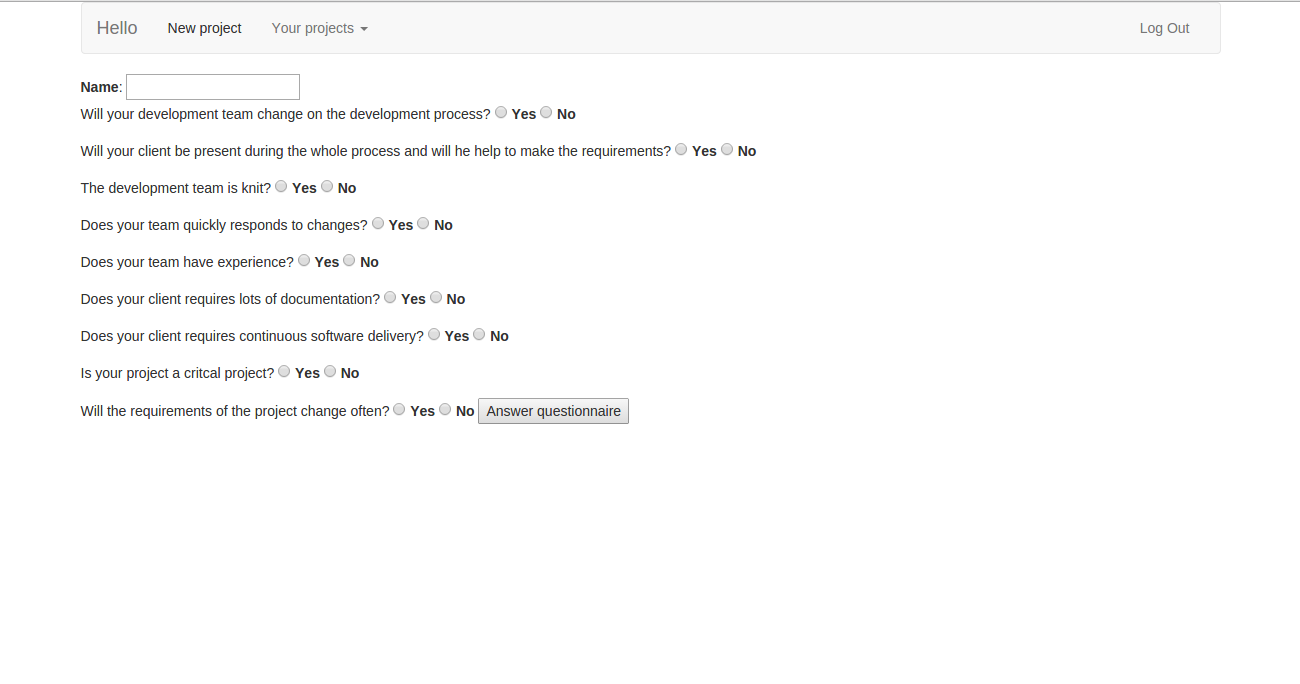
\includegraphics[scale=0.3]{imgFerramenta/questionarioBranco}
	\caption{Questionário antes do preenchimento}
	\label{img:questionario_antes}
\end{figure}

\begin{figure}[H]
	\centering
	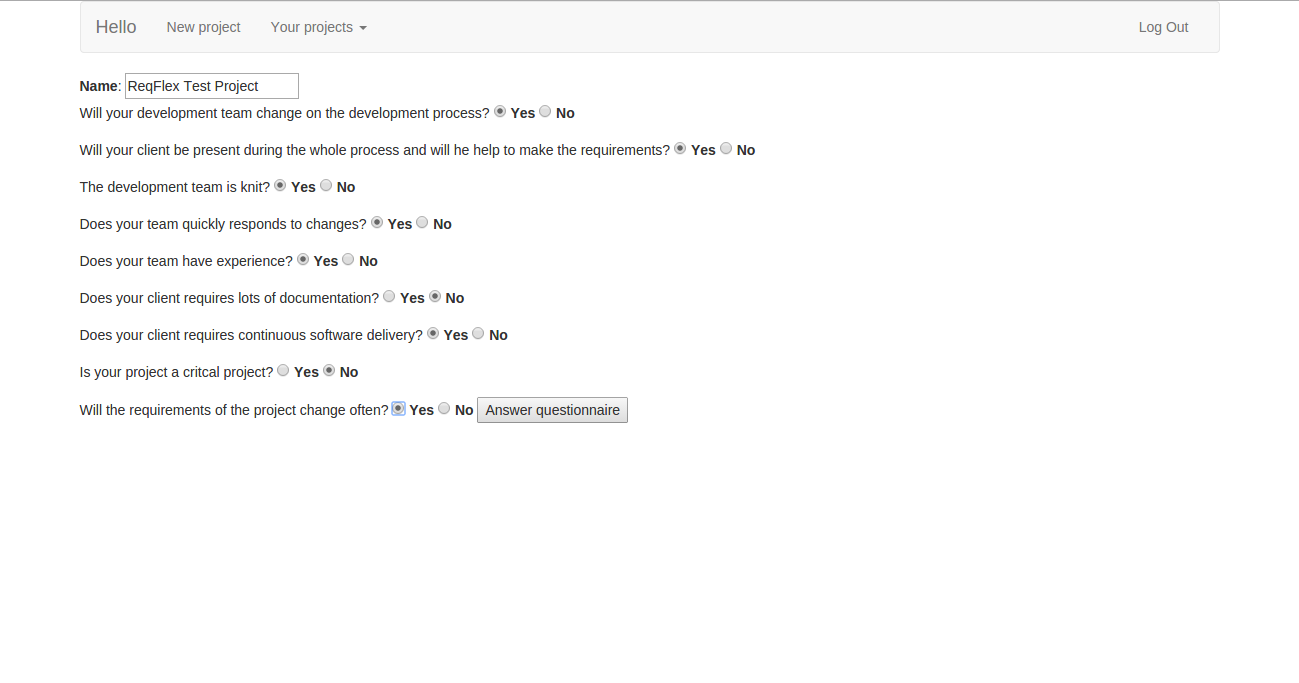
\includegraphics[scale=0.3]{imgFerramenta/questionarioPreenchido}
	\caption{Questionario antes do preenchimento}
	\label{img:questionario_depois}
\end{figure}

Após o usuário preencher e enviar o formulário o sistema computa suas respostas gerando uma lista de práticas que serão parte do processo do usuário. Estas práticas são listadas, e o usuário é indagado se está de acordo com o processo gerado para ele, assim com é apresentado na Figura \ref{img:result_questionario}.

Caso selecione que não o usuário será redirecionado para editar seu processo, caso aceite, será apresentado qual a rota final do projeto e suas práticas.

\begin{figure}[H]
	\centering
	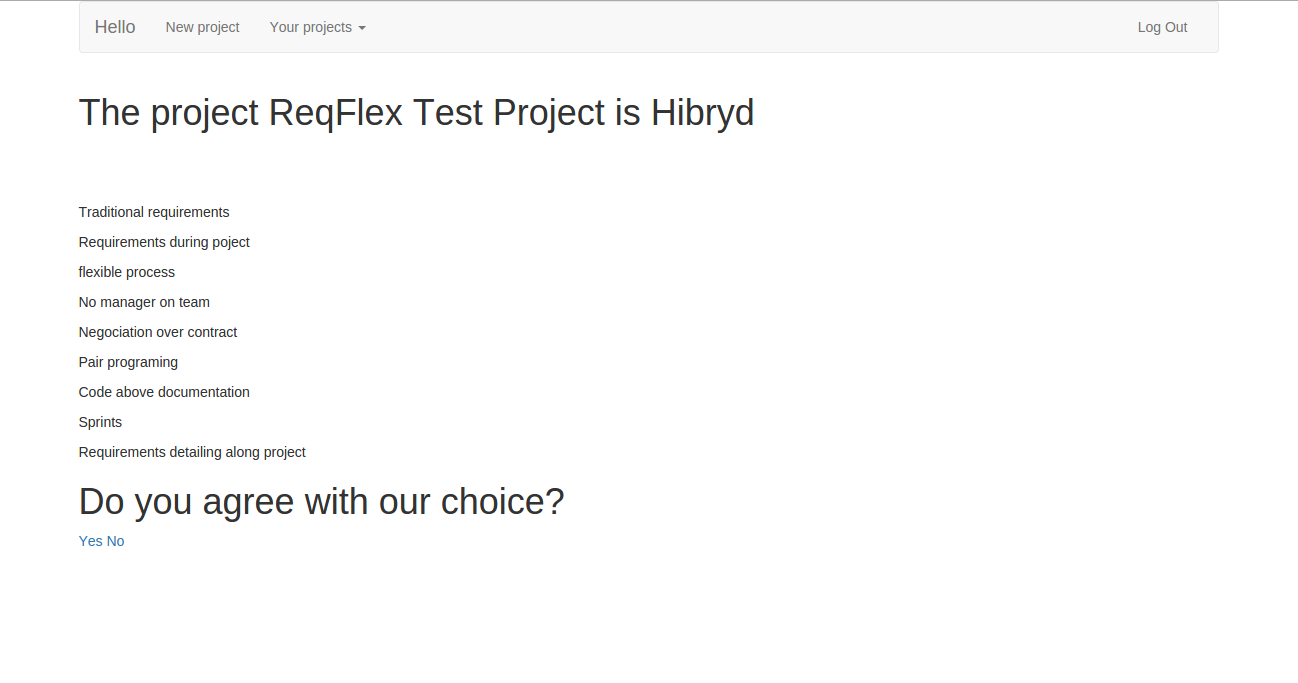
\includegraphics[scale=0.3]{imgFerramenta/resultadoQuestionario}
	\caption{Resultado do questionário}
	\label{img:result_questionario}
\end{figure}

No caso do usuário decidir que o processo montado para ele não está de acordo com suas preferências, serão apresentados todas as práticas que estão presentes no processo atual e a opção de trocá-las pelas práticas equivalentes na outra metodologia, ou apenas deletá-la se for o caso, como é mostrado na Figura \ref{img:questio_nao_aceito}.

Para poder caber a imagem no documento, foram retiradas várias práticas do processo a fim de mostrar toda a página.

\begin{figure}[H]
	\centering
	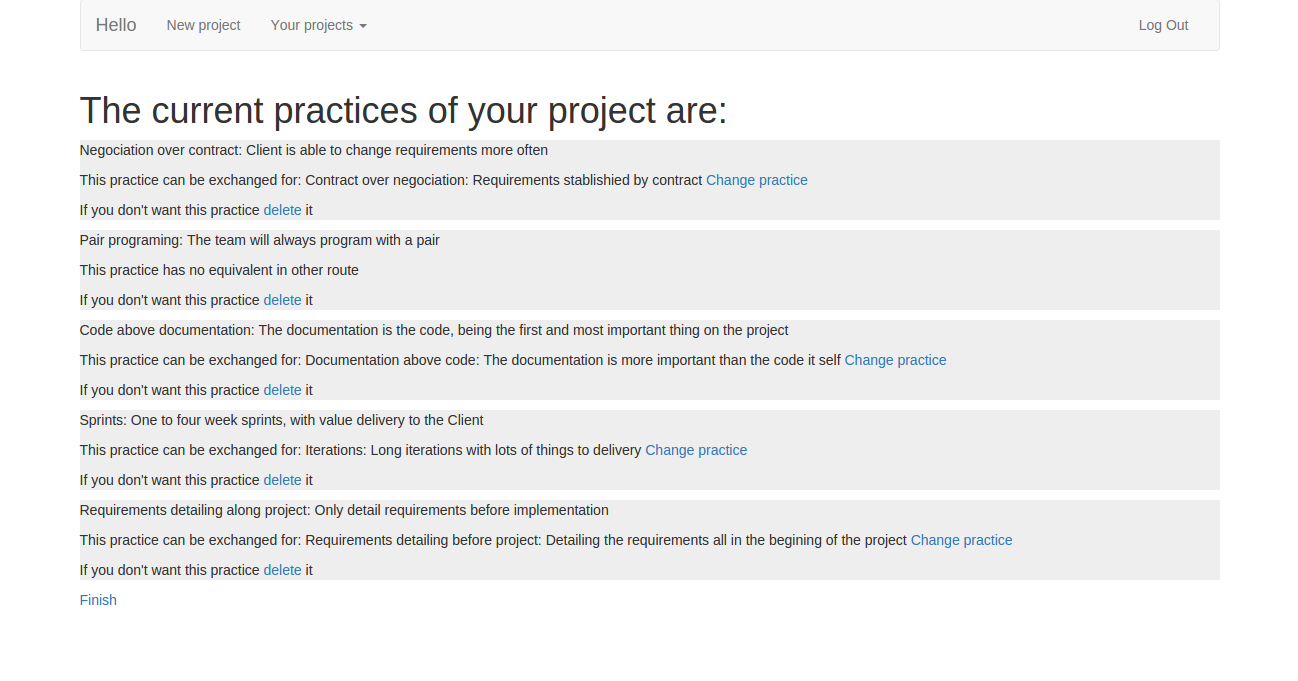
\includegraphics[scale=0.3]{imgFerramenta/edicaoQuestionario}
	\caption{Resultado não aceito}
	\label{img:questio_nao_aceito}
\end{figure}

Caso o usuário aceite o processo, ou após a edição do processo rejeitado, será redirecionado para a página que mostra todas as práticas, suas descrições e qual a rota que mais está sendo utilizada no processo, assim como mostra a Figura \ref{img:resultado_processo}.

\begin{figure}[H]
	\centering
	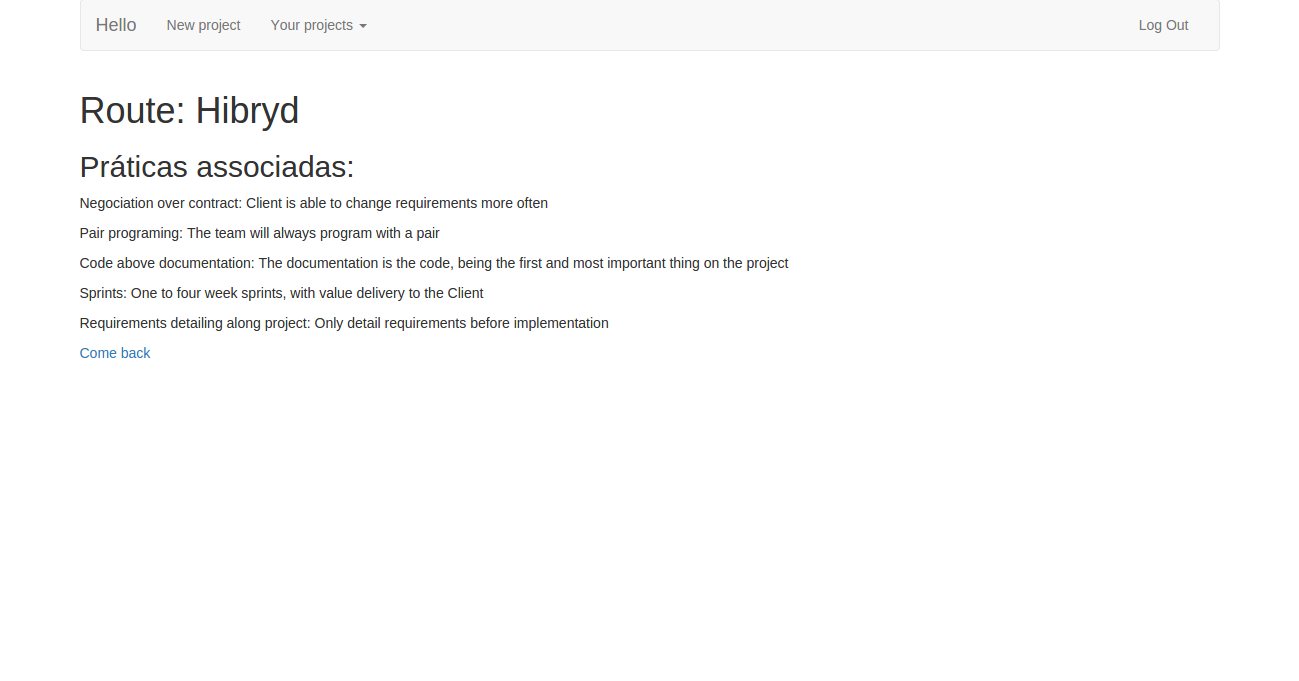
\includegraphics[scale=0.3]{imgFerramenta/resultado}
	\caption{Resultado final do processo}
	\label{img:resultado_processo}
\end{figure}

Finalmente após o processo aceito e visualizado pelo usuário, o sistema volta para o início, porém agora o processo criado está visível na aba ``\textit{Your projects}'', onde pode ser acessado a qualquer momento para ser consultado quais práticas devem ser seguidas, assim como é mostrado na Figura \ref{img:primeira_pag_dps}.

\begin{figure}[H]
	\centering
	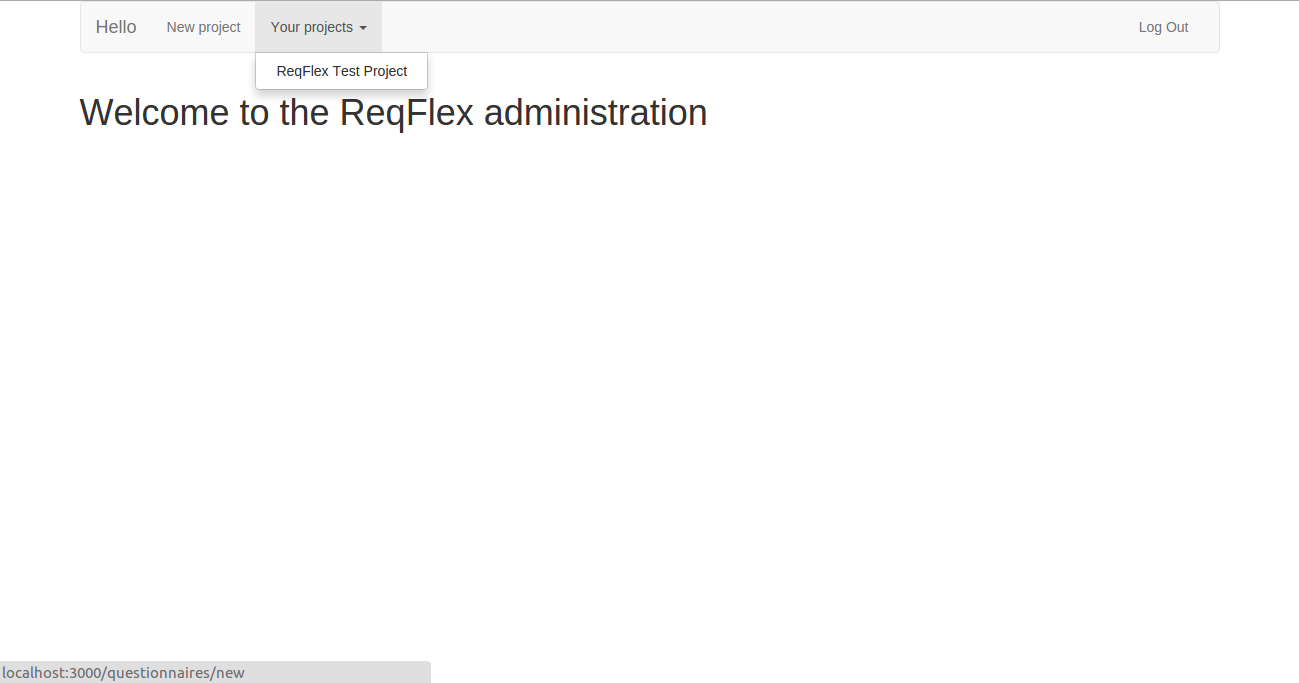
\includegraphics[scale=0.3]{imgFerramenta/primeiraPaginaDepois}
	\caption{Início depois do primeiro processo cadastrado}
	\label{img:primeira_pag_dps}
\end{figure}

\chapter{Relato de experiência}

O trabalho que gerou este documento foi uma experiência diferente de outros trabalhos ja realizados pela equipe, mesmo na mesma matéria em semestres anteriores, e em discução com a equipe foi percebido que o que mais influenciou para esta diferença toda foi uma proximidade maior com o professor devido a ele ser nosso cliente, diferentemente de outros grupos, ou até mesmo nós em semestres passados, que apenas recebiamos um texto para identificar o problema.

Esta diferença foi tanto boa quanto ruim em alguns aspectos, por exemplo de bom pudemos apresentar constantemente nossas angústias em relação ao tempo destinado à matéria, assim como sempre ter uma fonte 100\% segura para tirar nossas dúvidas sobre qualquer parte do problema, ou da própria matéria as vezes.

Infelizmente o trabalho também teve seus problemas, como não obtivemos um texto para retirar nossos requisitos, dependiamos de reuniões presenciais para poder realizar a elicitação e validação, sem poder supor que estavam certos, mesmo que o tema fosse de conhecimento da equipe, continuou sendo um tema complexo.

O maior dos problemas enfrentados pelo grupo não foi algo que a disciplina impôs, nem algo que pudesse ser contornado, que foi o fato de para o grupo, o tempo do trabalho estar reduzido por 1 semana devido a uma viagem de um dos membros da equipe, o que adiantou a entrega de dia 3 de dezembro para 25 de novembro, criando assim um desgaste muito grande em pouco tempo, porém tudo foi resolvido, apenas foi impossível terminar as duas fases de construção que estavam previstas inicialmente.

Outra grande dificuldade durante o trabalho não foi algo que foi imposto pela disciplina, porém escolhido pela equipe, foi a implementação, que foi realizada em uma linguagem desconhecida a todos os membros do desenvolvimento, e que exigiu boa parte do tempo, já curto, para aprendizagem.

No balanço geral o trabalho rendeu frutos positivos, possibilitando a toda a equipe um maior conhecimento tanto sobre a teoria sobre a \er~ quanto em relação a projetos reais, onde o cliente nem sempre está disponível a estar com a equipe, e mesmo assim ainda ter prazos de entregas, além de aprender tecnologias novas e funcionais para futuros projetos.

\chapter{Avaliação}

A avaliação presente neste apêndice é apenas uma avaliação da disciplina, devido ao fato da equipe não possuir uma equipe de MPR para acompanhá-la.

\begin{itemize}
	\item Avaliações positivas
		\begin{enumerate}
			\item A disciplina está com uma visão voltada a um projeto real;
			\item A disciplina proporciona a discução entre temas interessantes;
			\item A disciplina, para a nossa equipe, permitiu a escolha de quase tudo o que fizemos, possibilitando assim a oportuinidade de desenvolver senso crítico para alguns assuntos;
			\item A disciplina permitiu para a equipe um amadurecimento profissional, acadêmico e pessoal.
		\end{enumerate}

	\item Avaliações negativas
		\begin{enumerate}
			\item A disciplina está muito puxada, considerando ser uma matéria de 4 créditos, tendo um trabalho grande assim como provas de um nível razoável;
			\item Foram necessárias demasiadas reuniões com o professor fora do horário de aula, o que não era sempre possível para todos os membros devido a estágios e outros compromissos;
			\item Poucos pontos de controle e informações sobre o trabalho, não se aplica à equipe devido a reuniões constantes, porém aplica-se a quase todas as outras;
			\item Impossibilidade de recuperação caso haja uma nota ruim, uma nota baixa na prova 1 torna quase impossível a aprovação.
		\end{enumerate}
\end{itemize}

Infelizmente sabemos que os pontos negativos muitas pessoas que não tem interesse na matéria citam constantemente por não estarem dispostas a estar fazendo o trabalho além dos horários prédefinidos pelo plano de ensino, porém não foi o caso da equipe, tendo em vista que 3 dos 4 membros estagiam, e geralmente no horário que estavam marcados de atendimento.